\title{AIAA Technical Conference Paper Example}

% typeset with pdflatex, bibtex, pdflatex, pdflatex

\documentclass{aiaa-tc}

 \author{First M. Last%
         \thanks{Job Title, Department, Address, and AIAA Member Grade.}\\
         \normalsize\itshape
         Affiliation, City, Province, Zipcode, Country}

\begin{document}

\maketitle

\begin{abstract}
This is a bare-bones \LaTeX{} template of an AIAA technical conference paper.
It is intended to demonstrate the bare minimum set of \LaTeX{} commands
to produce an AIAA technical conference paper.
For detailed AIAA layout and style guidelines, please refer to the AIAA
author guide for paper submission, format, and other procedures.
\end{abstract}

\section*{Nomenclature}

 \begin{tabbing}
  XXX \= \kill % first line sets tab stop
  $J$ \> Jacobian Matrix \\
  $f$ \> Residual value vector \\
  $x$ \> Variable value vector \\
  $F$ \> Force, N \\
  $m$ \> Mass, kg \\
  $\Delta x$ \> Variable displacement vector \\
  $\alpha$ \> Acceleration, m/s\textsuperscript{2} \\[5pt]
  \textit{Subscript}\\
  $i$ \> Variable number \\
 \end{tabbing}

\section{Introduction}

This would be a good place to insert some text that make sense relative
to the paper being written.
Of course, for example purposes, the text is quite meaningless.

\subsection{Background}

This background section is here only to demonstrate \verb|\subsection| usage.
And following this, the next section level will need to be demonstrated.

\subsubsection{Detail}

Here is a \verb|\subsubsection| that would normally come in pairs of two
according to the requirements of an outline, but for the sake of
demonstration, we are only showing a single \verb|\subsubsection|.

\section{Model}

We should probably include some math.
Here we begin with Eq.~(\ref{e:function}) that demonstrates some math
typesetting.
\begin{equation}
 \label{e:function}
 \int_{0}^{r_{2}} F(r,\varphi) \, dr \, d\varphi =
    \left[ \sigma r_{2}/(2\mu_{0}) \right] \cdot
    \int_{0}^{\infty} \exp(-\rho|z_{j}-z_{i}|) \, \lambda^{-1} 
\end{equation}
Eq.~(\ref{e:function}) is grand.
Some say it is due to Sutton.\cite{sutton:85ar}

\section{Results}

In this section we will introduce some figures and tables.
It can be seen in figure~\ref{f:magnetic_field} that magnetization is a
function of applied field.
\begin{figure}
 \centering
 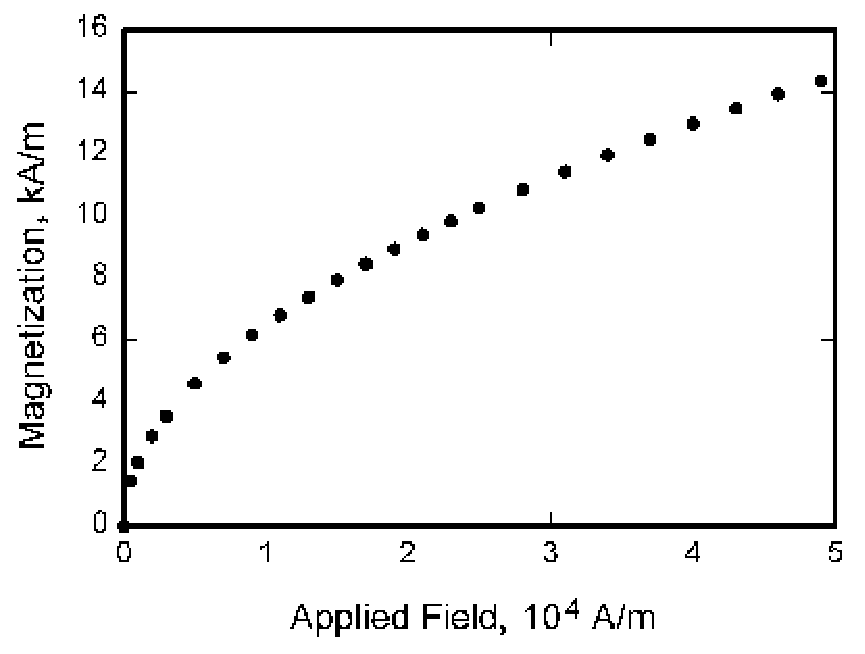
\includegraphics{figure}
 \caption{Magnetization as a function of applied field, which has
   borders so thick that they overwhelm the data and for some reason the
   ordinate label is rotated 90 degrees to make it difficult to
   read. This figure also demonstrates the dangers of using a bitmap
   as opposed to a vector image.}
 \label{f:magnetic_field}
\end{figure}
Sometimes writing meaningless text can be quiet easy, but other times
one is hard pressed to keep the words flowing.%
\footnote{And sometimes things get carried away in endless detail.}
Meanwhile back in the other world, table~\ref{t:scheme_comparison} shows
a nifty comparion.
\begin{table}
  \centering
  \caption{Variable and Fixed Coefficient Runge-Kutta Schemes as a
           Function of Reynolds Number}
  \label{t:scheme_comparison}
  \begin{tabular}{rrr}
       Re & Vary & Fixed \\\hline
        1 &  868 & 4,271 \\
       10 &  422 & 2,736 \\
       25 &  252 & 1,374 \\
       50 &  151 &   736 \\
      100 &  110 &   387 \\
      500 &   85 &   136 \\
    1,000 &   77 &   117 \\
    5,000 &   81 &    98 \\
   10,000 &   82 &    99
  \end{tabular}
\end{table}

\section{Conclusion}

After much typing, the paper can now conclude.
Four rocks were next to the channel.
This caused a few standing waves during the rip that one could ride on
the way in or jump on the way out.

\section*{Appendix}

An appendix, if needed, it should appear before the acknowledgments.
Use the 'starred' version of the \verb|\section| commands to avoid
section numbering.

\section*{Acknowledgments}

A place to recognize others or simply thank Kleb and Wood for this template.

\bibliographystyle{aiaa}
\bibliography{references}

\end{document}
